\noindent The schematic of the L-pad $1^{st}$ shunt attenuator is shown in Fig. \ref{fig:l-pad-shunt-attenuator-schematic} and its design equations are derived as follows using basic network analysis:

  \begin{figure}[ht]
    \centering
    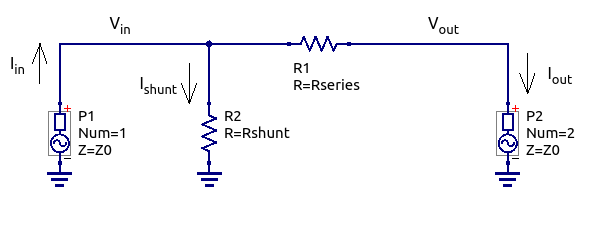
\includegraphics[width=10cm]{./images/l-pad-shunt-attenuator-schematic.png}
    \caption{L-pad shunt attenuator}
    \label{fig:l-pad-shunt-attenuator-schematic}
  \end{figure}
  
\begin{equation}
	\frac{V_{in} - V_{out}}{R_{series}} = \frac{V_{out}}{Z_0} \Rightarrow A_v = \sqrt{\alpha^{n.u.}} = \frac{V_{out}}{V_{in}} = \frac{Z_0}{Z_0 + R_{series}}
\end{equation}

\noindent Consequently,

\begin{equation}
	R_{series} = Z_0 \cdot \frac{1 - \sqrt{\alpha^{n.u.}}}{\sqrt{\alpha^{n.u.}}}
\end{equation}

\noindent The input port must be matched to $Z_0$, so:

\begin{equation}
	Z_0 = R_{shunt} \parallel R_{series} + Z_0 \Rightarrow R_{shunt} = Z_0 \cdot \frac{1}{1 - \sqrt{\alpha^{n.u.}}}
\end{equation}

\noindent The output impedance of the L-pad is, then:

\begin{equation}
	Z_{out} = R_{series} + R_{shunt} \parallel Z_0 = - Z_0 \cdot \frac{\alpha^{n.u.} - 2 \cdot \sqrt{\alpha^{n.u.}} + 2}{\alpha^{n.u.} - 2 \cdot \sqrt{\alpha^{n.u.}}}
\end{equation}

\noindent Concerning the power dissipation in the resistors, the corresponding equations for the shunt and the series resistors were found to be:

\begin{equation}
	P_{diss}^{shunt} = P_{in} \cdot \left( 1 - \sqrt{\alpha^{n.u.}}\right)
\end{equation}

\begin{equation}
	P_{diss}^{series} = P_{in} \cdot \sqrt{\alpha^{n.u.}} \cdot \frac{1 - 2 \cdot \sqrt{\alpha^{n.u.}} + \alpha}{1 - \sqrt{\alpha^{n.u.}}}
\end{equation}
  

